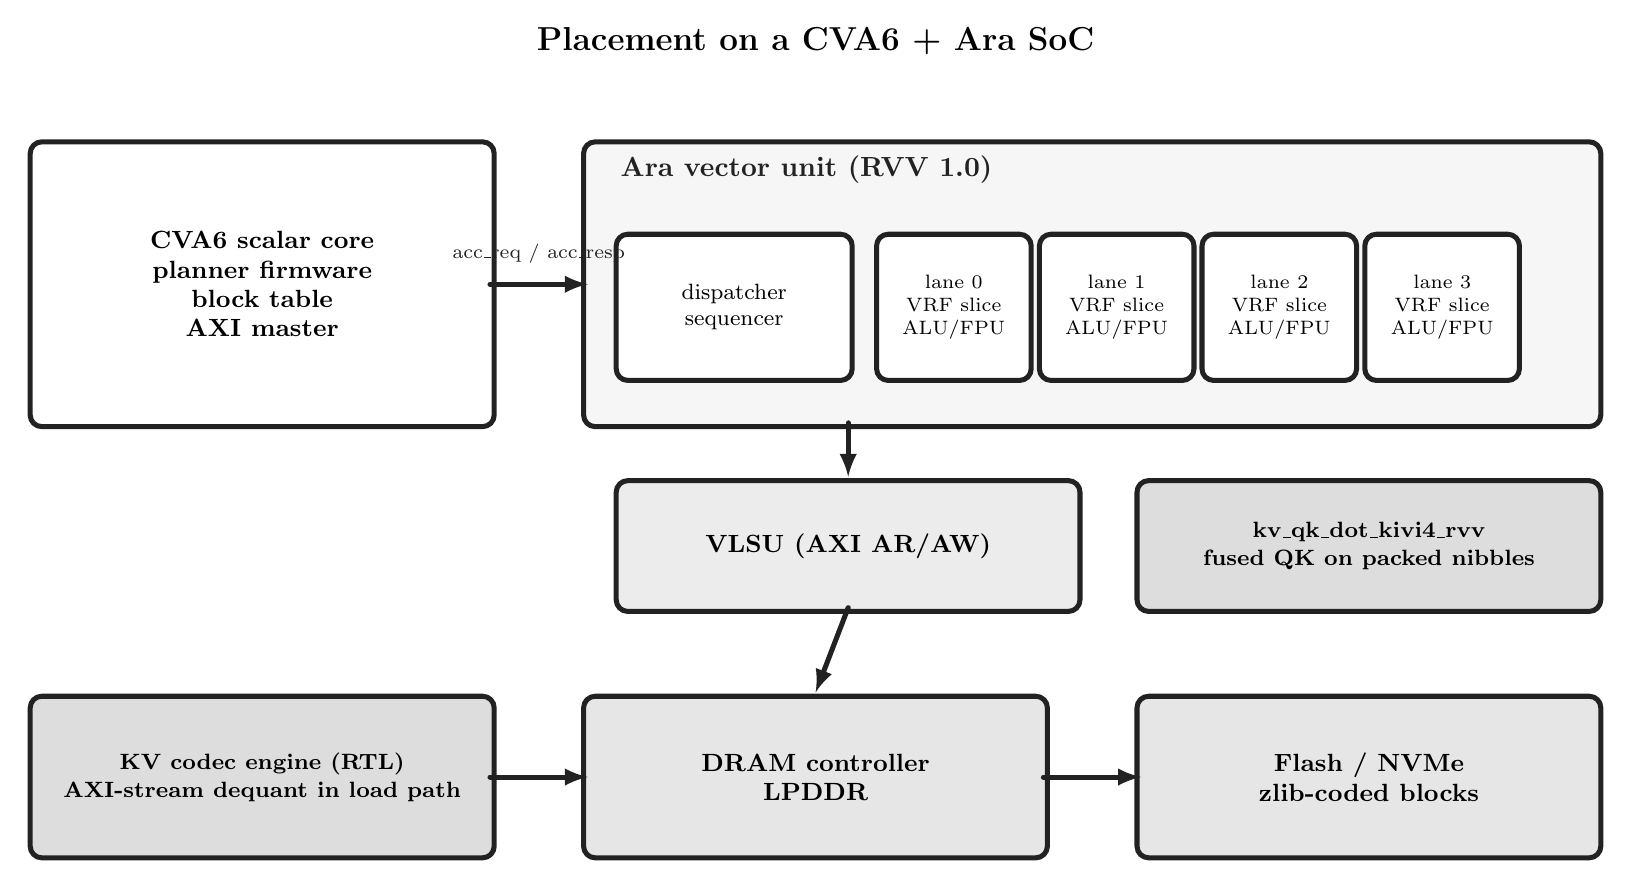
\begin{tikzpicture}[line cap=round,line join=round]
\draw[rounded corners=4.2pt,line width=1.82pt,draw={rgb,255:red,34;green,34;blue,34},fill={rgb,255:red,255;green,255;blue,255}] (0.142in,3.061in) rectangle (2.462in,4.485in);
\draw[rounded corners=4.2pt,line width=1.82pt,draw={rgb,255:red,34;green,34;blue,34},fill={rgb,255:red,246;green,246;blue,246}] (2.909in,3.061in) rectangle (7.995in,4.485in);
\draw[rounded corners=4.2pt,line width=1.82pt,draw={rgb,255:red,34;green,34;blue,34},fill={rgb,255:red,255;green,255;blue,255}] (3.072in,3.292in) rectangle (4.252in,4.023in);
\draw[rounded corners=4.2pt,line width=1.82pt,draw={rgb,255:red,34;green,34;blue,34},fill={rgb,255:red,255;green,255;blue,255}] (4.374in,3.292in) rectangle (5.147in,4.023in);
\draw[rounded corners=4.2pt,line width=1.82pt,draw={rgb,255:red,34;green,34;blue,34},fill={rgb,255:red,255;green,255;blue,255}] (5.188in,3.292in) rectangle (5.961in,4.023in);
\draw[rounded corners=4.2pt,line width=1.82pt,draw={rgb,255:red,34;green,34;blue,34},fill={rgb,255:red,255;green,255;blue,255}] (6.001in,3.292in) rectangle (6.774in,4.023in);
\draw[rounded corners=4.2pt,line width=1.82pt,draw={rgb,255:red,34;green,34;blue,34},fill={rgb,255:red,255;green,255;blue,255}] (6.815in,3.292in) rectangle (7.588in,4.023in);
\draw[rounded corners=4.2pt,line width=1.82pt,draw={rgb,255:red,34;green,34;blue,34},fill={rgb,255:red,236;green,236;blue,236}] (3.072in,2.137in) rectangle (5.391in,2.791in);
\draw[rounded corners=4.2pt,line width=1.82pt,draw={rgb,255:red,34;green,34;blue,34},fill={rgb,255:red,221;green,221;blue,221}] (5.676in,2.137in) rectangle (7.995in,2.791in);
\draw[rounded corners=4.2pt,line width=1.82pt,draw={rgb,255:red,34;green,34;blue,34},fill={rgb,255:red,221;green,221;blue,221}] (0.142in,0.905in) rectangle (2.462in,1.713in);
\draw[rounded corners=4.2pt,line width=1.82pt,draw={rgb,255:red,34;green,34;blue,34},fill={rgb,255:red,230;green,230;blue,230}] (2.909in,0.905in) rectangle (5.228in,1.713in);
\draw[rounded corners=4.2pt,line width=1.82pt,draw={rgb,255:red,34;green,34;blue,34},fill={rgb,255:red,230;green,230;blue,230}] (5.676in,0.905in) rectangle (7.995in,1.713in);
\draw[-latex,line width=1.82pt,draw={rgb,255:red,34;green,34;blue,34}] (2.441in,3.773in) -- (2.930in,3.773in);
\draw[-latex,line width=1.82pt,draw={rgb,255:red,34;green,34;blue,34}] (4.232in,2.156in) -- (4.069in,1.732in);
\draw[-latex,line width=1.82pt,draw={rgb,255:red,34;green,34;blue,34}] (2.441in,1.309in) -- (2.930in,1.309in);
\draw[-latex,line width=1.82pt,draw={rgb,255:red,34;green,34;blue,34}] (5.208in,1.309in) -- (5.696in,1.309in);
\draw[-latex,line width=1.82pt,draw={rgb,255:red,34;green,34;blue,34}] (4.232in,3.080in) -- (4.232in,2.810in);
\node[align=center,text={rgb,255:red,0;green,0;blue,0},font=\fontsize{9.0pt}{10.6pt}\selectfont\bfseries,inner sep=0pt] at (1.302in,3.773in) {CVA6 scalar core \\ planner firmware \\ block table \\ AXI master};
\node[anchor=south west,align=left,text={rgb,255:red,34;green,34;blue,34},font=\fontsize{10.0pt}{11.8pt}\selectfont\bfseries,inner sep=0pt] at (3.092in,4.274in) {Ara vector unit (RVV 1.0)};
\node[align=center,text={rgb,255:red,0;green,0;blue,0},font=\fontsize{8.0pt}{9.4pt}\selectfont,inner sep=0pt] at (3.662in,3.657in) {dispatcher \\ sequencer};
\node[align=center,text={rgb,255:red,0;green,0;blue,0},font=\fontsize{7.0pt}{8.3pt}\selectfont,inner sep=0pt] at (4.760in,3.657in) {lane 0 \\ VRF slice \\ ALU/FPU};
\node[align=center,text={rgb,255:red,0;green,0;blue,0},font=\fontsize{7.0pt}{8.3pt}\selectfont,inner sep=0pt] at (5.574in,3.657in) {lane 1 \\ VRF slice \\ ALU/FPU};
\node[align=center,text={rgb,255:red,0;green,0;blue,0},font=\fontsize{7.0pt}{8.3pt}\selectfont,inner sep=0pt] at (6.388in,3.657in) {lane 2 \\ VRF slice \\ ALU/FPU};
\node[align=center,text={rgb,255:red,0;green,0;blue,0},font=\fontsize{7.0pt}{8.3pt}\selectfont,inner sep=0pt] at (7.202in,3.657in) {lane 3 \\ VRF slice \\ ALU/FPU};
\node[align=center,text={rgb,255:red,0;green,0;blue,0},font=\fontsize{9.0pt}{10.6pt}\selectfont\bfseries,inner sep=0pt] at (4.232in,2.464in) {VLSU (AXI AR/AW)};
\node[align=center,text={rgb,255:red,0;green,0;blue,0},font=\fontsize{8.5pt}{10.0pt}\selectfont\bfseries,inner sep=0pt] at (6.836in,2.464in) {kv\_qk\_dot\_kivi4\_rvv \\ fused QK on packed nibbles};
\node[align=center,text={rgb,255:red,0;green,0;blue,0},font=\fontsize{8.5pt}{10.0pt}\selectfont\bfseries,inner sep=0pt] at (1.302in,1.309in) {KV codec engine (RTL) \\ AXI-stream dequant in load path};
\node[align=center,text={rgb,255:red,0;green,0;blue,0},font=\fontsize{9.0pt}{10.6pt}\selectfont\bfseries,inner sep=0pt] at (4.069in,1.309in) {DRAM controller \\ LPDDR};
\node[align=center,text={rgb,255:red,0;green,0;blue,0},font=\fontsize{9.0pt}{10.6pt}\selectfont\bfseries,inner sep=0pt] at (6.836in,1.309in) {Flash / NVMe \\ zlib-coded blocks};
\node[align=center,text={rgb,255:red,34;green,34;blue,34},font=\fontsize{7.5pt}{8.8pt}\selectfont,inner sep=0pt] at (2.685in,3.927in) {acc\_req / acc\_resp};
\node[anchor=south,align=center,text={rgb,255:red,0;green,0;blue,0},font=\fontsize{12.0pt}{14.2pt}\selectfont\bfseries,inner sep=0pt] at (4.069in,4.917in) {Placement on a CVA6 + Ara SoC};
\end{tikzpicture}
